% Options for packages loaded elsewhere
\PassOptionsToPackage{unicode}{hyperref}
\PassOptionsToPackage{hyphens}{url}
\PassOptionsToPackage{dvipsnames,svgnames*,x11names*}{xcolor}
%
\documentclass[
  10pt,
  ignorenonframetext,
  x11names, dvipsnames, bibspacing, natbib, table]{beamer}
\usepackage{pgfpages}
\setbeamertemplate{caption}[numbered]
\setbeamertemplate{caption label separator}{: }
\setbeamercolor{caption name}{fg=normal text.fg}
\beamertemplatenavigationsymbolsempty
% Prevent slide breaks in the middle of a paragraph
\widowpenalties 1 10000
\raggedbottom
\setbeamertemplate{part page}{
  \centering
  \begin{beamercolorbox}[sep=16pt,center]{part title}
    \usebeamerfont{part title}\insertpart\par
  \end{beamercolorbox}
}
\setbeamertemplate{section page}{
  \centering
  \begin{beamercolorbox}[sep=12pt,center]{part title}
    \usebeamerfont{section title}\insertsection\par
  \end{beamercolorbox}
}
\setbeamertemplate{subsection page}{
  \centering
  \begin{beamercolorbox}[sep=8pt,center]{part title}
    \usebeamerfont{subsection title}\insertsubsection\par
  \end{beamercolorbox}
}
\AtBeginPart{
  \frame{\partpage}
}
\AtBeginSection{
  \ifbibliography
  \else
    \frame{\sectionpage}
  \fi
}
\AtBeginSubsection{
  \frame{\subsectionpage}
}
\usepackage{amsmath,amssymb}
\usepackage{lmodern}
\usepackage{ifxetex,ifluatex}
\ifnum 0\ifxetex 1\fi\ifluatex 1\fi=0 % if pdftex
  \usepackage[T1]{fontenc}
  \usepackage[utf8]{inputenc}
  \usepackage{textcomp} % provide euro and other symbols
\else % if luatex or xetex
  \usepackage{unicode-math}
  \defaultfontfeatures{Scale=MatchLowercase}
  \defaultfontfeatures[\rmfamily]{Ligatures=TeX,Scale=1}
\fi
\usetheme[]{Rafal_beamerSly1}
% Use upquote if available, for straight quotes in verbatim environments
\IfFileExists{upquote.sty}{\usepackage{upquote}}{}
\IfFileExists{microtype.sty}{% use microtype if available
  \usepackage[]{microtype}
  \UseMicrotypeSet[protrusion]{basicmath} % disable protrusion for tt fonts
}{}
\makeatletter
\@ifundefined{KOMAClassName}{% if non-KOMA class
  \IfFileExists{parskip.sty}{%
    \usepackage{parskip}
  }{% else
    \setlength{\parindent}{0pt}
    \setlength{\parskip}{6pt plus 2pt minus 1pt}}
}{% if KOMA class
  \KOMAoptions{parskip=half}}
\makeatother
\usepackage{xcolor}
\IfFileExists{xurl.sty}{\usepackage{xurl}}{} % add URL line breaks if available
\IfFileExists{bookmark.sty}{\usepackage{bookmark}}{\usepackage{hyperref}}
\hypersetup{
  pdftitle={Taking uncertainty seriously A Bayesian approach to word embedding bias estimation},
  pdfauthor={Alicja Dobrzeniecka \& Rafal Urbaniak (LoPSE research group, University of Gdansk)},
  colorlinks=true,
  linkcolor=Maroon,
  filecolor=Maroon,
  citecolor=Blue,
  urlcolor=blue,
  pdfcreator={LaTeX via pandoc}}
\urlstyle{same} % disable monospaced font for URLs
\newif\ifbibliography
\setlength{\emergencystretch}{3em} % prevent overfull lines
\providecommand{\tightlist}{%
  \setlength{\itemsep}{0pt}\setlength{\parskip}{0pt}}
\setcounter{secnumdepth}{-\maxdimen} % remove section numbering
\ifluatex
  \usepackage{selnolig}  % disable illegal ligatures
\fi

\title{\Large Taking uncertainty seriously \newline \normalsize A
Bayesian approach to word embedding bias estimation}
\author{Alicja Dobrzeniecka \& Rafal Urbaniak
\footnotesize \newline (LoPSE research group, University of Gdansk)}
\date{Boston, April Fools' Day}

\begin{document}
\frame{\titlepage}

\begin{frame}{Cosine similarity}
\protect\hypertarget{cosine-similarity}{}
\begin{columns}
\column{0.45\linewidth}
    

\begin{center}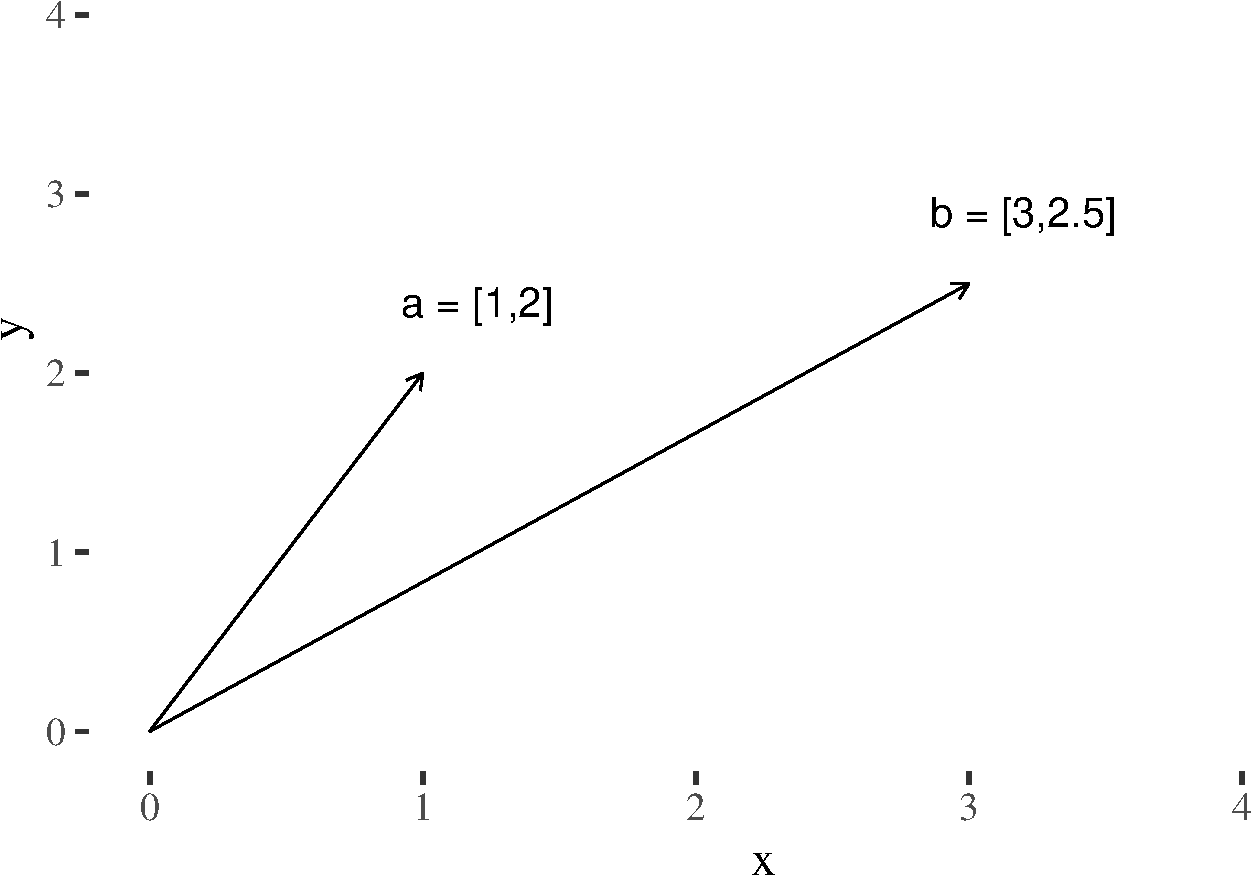
\includegraphics[width=1\linewidth]{tryOut_files/figure-beamer/cosine1-1} \end{center}


\column{0.5\linewidth}

\footnotesize 

\begin{block}{Vectors}
\begin{align*}
a  & = [1,2]\\
b  &= [3,2]
\end{align*}

\end{block}
\pause 

\begin{block}{Dot product}


\begin{align*}
a \cdot b & = a_1 b_1 + a_2 b_2\\
a \cdot a & = a_1^2 + a_2 ^ 2 \\
\lVert a\rVert & = \sqrt(a \cdot a)
\end{align*}

\end{block}



\end{columns}
\end{frame}

\begin{frame}{Cosine similarity}
\protect\hypertarget{cosine-similarity-1}{}
\begin{columns}
\column{0.45\linewidth}
    

\begin{center}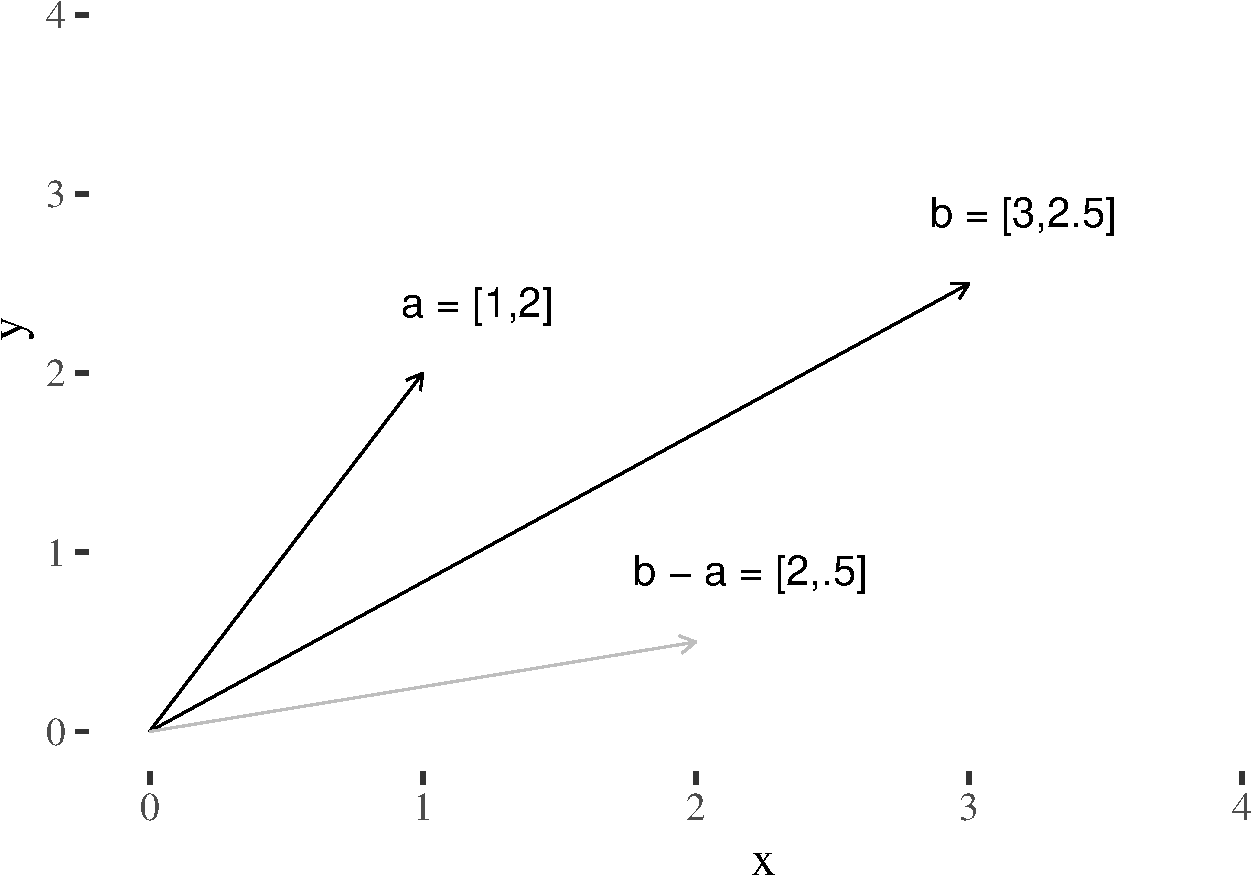
\includegraphics[width=1\linewidth]{tryOut_files/figure-beamer/cosine2-1} \end{center}


\column{0.5\linewidth}

\footnotesize 


\begin{block}{Vectors}

\begin{align*}
a  & = [1,2]\\
b  &= [4,4]
\end{align*}

\end{block}


\begin{block}{Dot product}

\begin{align*}
a \cdot b & = a_1 b_1 + a_2 b_2\\
a \cdot a & = a_1^2 + a_2 ^ 2 \\
\lVert a\rVert & = \sqrt(a \cdot a)
\end{align*}

\end{block}


\begin{block}{Vector difference}

\begin{align*}
b - a & = [b_1- a_1, b_2 - a_2 ]
\end{align*}

\end{block}

\end{columns}
\end{frame}

\begin{frame}{Cosine similarity}
\protect\hypertarget{cosine-similarity-2}{}
\begin{columns}
\column{0.45\linewidth}
    

\begin{center}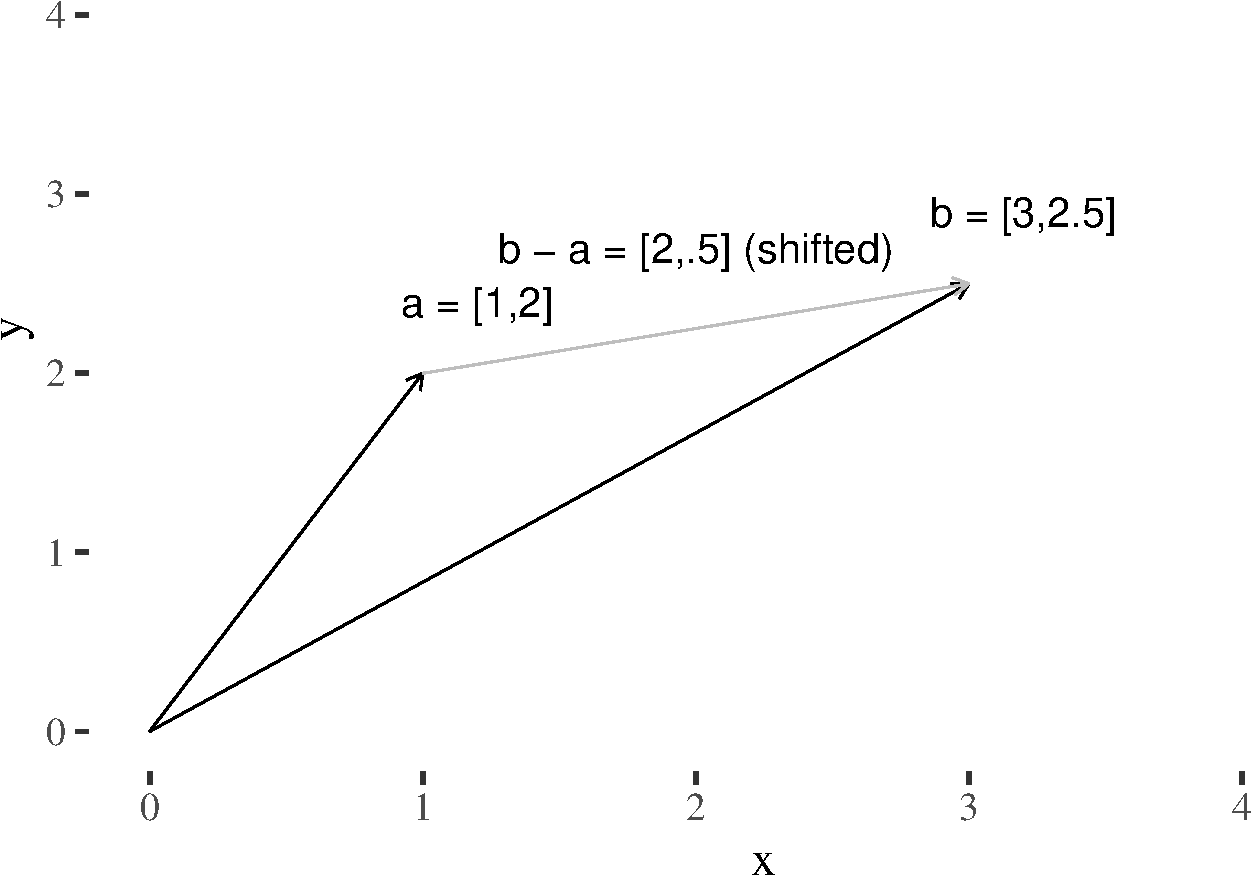
\includegraphics[width=1\linewidth]{tryOut_files/figure-beamer/cosine3-1} \end{center}



\column{0.5\linewidth}

\footnotesize 


\begin{block}{Vectors}

\begin{align*}
a  & = [1,2]\\
b  &= [4,4]
\end{align*}

\end{block}


\begin{block}{Dot product}

\begin{align*}
a \cdot b & = a_1 b_1 + a_2 b_2\\
a \cdot a & = a_1^2 + a_2 ^ 2 \\
\lVert a\rVert & = \sqrt(a \cdot a)
\end{align*}

\end{block}


\begin{block}{Vector difference}

\begin{align*}
b - a & = [b_1- a_1, b_2 - a_2 ]
\end{align*}

\end{block}

\end{columns}
\end{frame}

\begin{frame}{Cosine similarity}
\protect\hypertarget{cosine-similarity-3}{}
\begin{columns}
\column{0.45\linewidth}
    

\begin{center}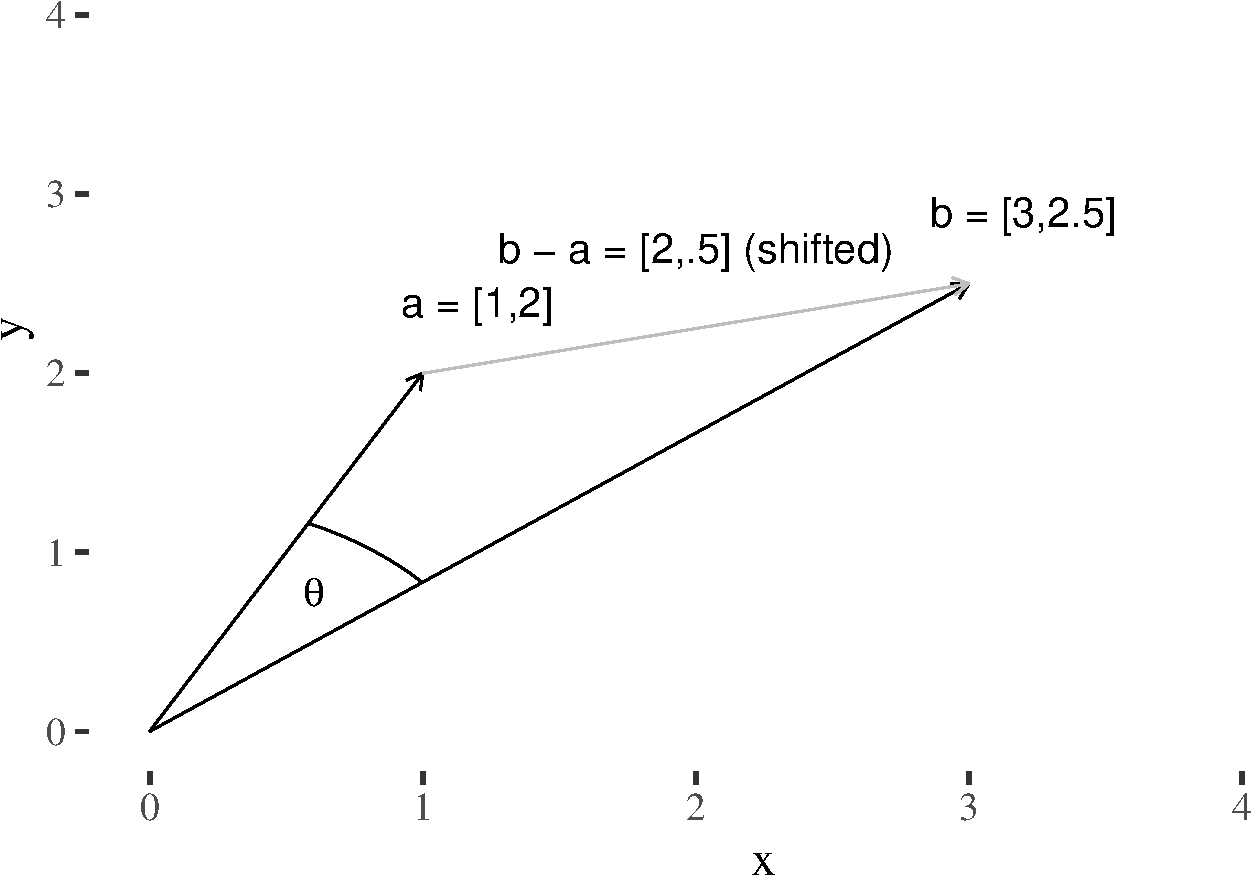
\includegraphics[width=1\linewidth]{tryOut_files/figure-beamer/cosine4-1} \end{center}



\column{0.5\linewidth}

\footnotesize 


\begin{block}{Angle}

\begin{align*}
\lVert b - a \rVert^2 &  = \lVert  b \rVert^2 + \lVert a \rVert^2 - 
  2 \lVert b \rVert   \lvert  a \rVert  \cos \theta  \\
b \cdot a  & = \lVert b\rVert \lVert  a \rVert \cos \theta \\ 
\cos \theta & = \frac{b \cdot a}{\lVert b\rVert  \lVert  a \rVert }
\end{align*}

\end{block}


\pause 

\begin{block}{Orthogonality}
\begin{align*}
\cos ( 90^{\circ}) & = 0 \\ 
\frac{b \cdot a}{\lVert  b\rVert \lVert a \rVert} & = 0\\ 
 b \cdot a & = 0  
\end{align*}
\end{block}







\end{columns}
\end{frame}

\end{document}
